\documentclass[conference]{IEEEtran}
\IEEEoverridecommandlockouts
\usepackage{cite}
\usepackage{amsmath,amssymb,amsfonts}
\usepackage{algorithmic}
\usepackage{mathpazo}
\usepackage[spanish]{babel}
\usepackage[utf8]{inputenc}
\usepackage{graphicx}
\usepackage{textcomp}
\usepackage{xcolor}
%\usepackage{minted}
%\usemintedstyle{emacs}
\usepackage{url}
\usepackage{ctable}
\usepackage{float}
\usepackage{amsmath,amssymb,amsfonts}
\usepackage{makecell}
\usepackage{hyperref}
\usepackage{comment}
\hypersetup{
	colorlinks=true,
	linkcolor=blue,
	filecolor=magenta,      
	urlcolor=cyan,
}
\newcommand{\DNoise}{n_d}

\newcommand{\Est}[1]{\hat{#1}}
\newcommand{\Test}[1]{\expandafter\hat#1}

\def\BibTeX{{\rm B\kern-.05em{\sc i\kern-.025em b}\kern-.08em
    T\kern-.1667em\lower.7ex\hbox{E}\kern-.125emX}}
    
\begin{document}
\title{\bf{Adaptación de los personajes del anime de One Punch man a una estructura RDF}}


\author{\IEEEauthorblockN{Diego Bergna Aguilar}
\IEEEauthorblockA{\textit{Universidad Nacional de Ingenier\'ia} \\
Lima, Per\'u \\
\texttt{diego.bergna.a@uni.pe}}
\\
\IEEEauthorblockN{Italo Silva Guanilo}
\IEEEauthorblockA{\textit{Universidad Nacional de Ingenier\'ia} \\
Lima, Perú \\
\texttt{italosilva@uni.pe}}
\and
\IEEEauthorblockN{Stefano Olivieri Romero}
\IEEEauthorblockA{\textit{Universidad Nacional de Ingenier\'ia} \\
Lima, Perú \\
\texttt{solivierir@uni.pe}}
\\
\IEEEauthorblockN{Kevin Paima Mijahuanca}
\IEEEauthorblockA{\textit{Universidad Nacional de Ingenier\'ia} \\
Lima, Perú \\
\texttt{kpaimam@uni.pe}}}

\maketitle

\begin{abstract}

La Web Semántica se basa en la idea del uso de tecnologías  para la publicación de datos que sean legibles por aplicaciones informáticas.
Se basa en la adición de metadatos semánticos y ontológicos a la World Wide Web. Uno de los métodos empleados para lograr esto es el llamado RDF (Resource Description Framework por sus siglas en inglés).

En este trabajo de investigación se usaron los conceptos de RDF sobre una base de datos para transformarla tablas de Triples y luego poder realizar una serie de acciones sobre ella con el fin de comprender mejor las ventajas y usos de la aplicación de RDF.

\vspace{0.2cm}

\'Indice de T\'erminos— RDF, owl, Web Semántica, triples, URI.
    
\end{abstract}

\section{Introducción}

Una de las características de la Web Semántica es el lema AAA: $"$Anyone can say Anything about Any topic$"$ lo que en español quiere decir: 
$"$Cualquiera puede decir cualquier cosa sobre cualquier tema$"$. 
Entonces en una red de información cualquiera debe poder aportar conocimiento sobre un recurso. 
De esta manera tendremos la información distribuida en varias fuentes.

El reto para implementar la Web Semántica estuvo en implementar un modelo de datos que permita la distribución de información a través de la Web.
Esto se logra con el modelo de datos llamado \texttt{Resource Description Framework (RDF)}.

El presente trabajo busca construir una estructura RDF basada en una \texttt{Wiki} de una animación japonesa y manipularla para describir los recursos en un dominio determinado, reconocer los beneficios de la Web Semántica.



%Los datos suelen representarse en forma tabular, en la que las filas representan los elementos que estamos describiendo y las columnas representan a sus propiedades.
%Entonces cada celda de la tabla vienen a ser los valores particulares de estas propiedades.

\section{Estructura RDF}

RDF son las siglas de Resource Description Framework (Marco de descripción de recursos) el cual es un modelo que usa un formato sujeto-predicado-objeto, la cual es una forma estandarizada de describir las cosas.

Dado que una celda se representa con tres valores, el bloque de construcción básico para RDF se llama Triple en el cual el identificador de la fila se llama sujeto, al identificador de la columna se le llama predicado; mientras que al valor de la celda se le llama objeto del triple.



La siguiente tabla expresa los triples como sujeto, predicado y objeto; además, muestra cuando más de un triple hace referencia a la misma entidad.

\begin{table}[H]
\begin{center}
\begin{tabular}{|c|c|c|}
\textbf{Subject}& \textbf{Predicate} & \textbf{Object}  \\
     Saitama & es & Héroe \\
     Orochi & es & Monstruo\\
     Boros & es & Alien \\
     Genos & es & Héroe \\
     Genos & vive en & Ciudad Z \\
     Saitama & vive en & Ciudad Z
\end{tabular}
\end{center}
\caption{Ejemplos de Triples con más de una referencia a una misma entidad.}
\end{table}


De esta manera nos percatamos que es conveniente interpretar a los Triples como grafos dirigidos en los que cada triple es un nodo enlazado por su sujeto y su predicado.

\begin{figure}[H]
\centering
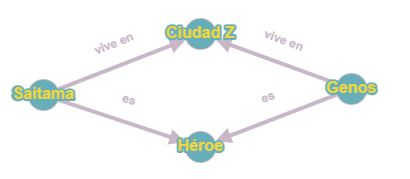
\includegraphics[scale=0.7]{img/G - 01.JPG} 
\caption{Grafo de la tabla anterior.}
\end{figure}



\subsection{Fusión de datos de múltiples fuentes}

Para usar esta información distribuida es necesario fusionar las diversas fuentes.
Para ello el proceso se resume en formar los grafos de los triples y combinarlos respetando el sujeto-predicado de cada objeto.

\subsection{Espacios de nombres, URIS e Identidad}

El poder fusionar correctamente las distintas Triples que hay se reduce a solucionar la pregunta de \textbf{\textit{¿Cuándo un nodo en un grafo representa lo mismo que un nodo en otro grafo?}}

Dado que la información en la Web es abundante, se hace difícil que una sola palabra haga referencia a una única entidad; entonces, ¿Cómo resolvemos este inconveniente?

RDF emplea la solución llamada \texttt{URI} la cual es propia de la tecnología web fundamental.
Los URIs son identificadores para los recursos web.

Un URI proporciona una identificación a un recurso común en la Web. Como ejemplo si dos agentes hacen referencia a un mismo recurso, la práctica recomendada en la Web es que acepten un URI común para ese recurso.

Pero la ventaja de la URI es que se hace posible $"$desreferenciarlo$"$ obteniendo así toda la información en el URI, la cual indica cosas como nombre del servidor, protocolo, número de puerto, nombre de archivo, etc.
 lo cual permite localizar un archivo en la Web.
 
 Esto aplicado en RDF viene a darse como la fusión de un nodo de un grafo con otro nodo perteneciente a otro grafo siempre que ambos tengan el mismo URI.
 Como dato extra, esta solución no solo se aplica en la Web Semántica, sino en la Web en general.

\subsection{Expresando URIs en impresión}

Es tedioso tener que expresar los URI de manera impresa. La solución a esto es utilizar la versión simplificada de un esquema de abreviaturas URI las cuales se llaman \textit{qnames}.

De esta manera un URI al ser expresado en \textit{qname} contiene dos partes: un \textit{namespace} y un \textit{identificador} los que estan separados por dos puntos; por ejemplo, si escogemos el \textit{identificador} England en el \textit{namespace} geo, se denotará simplemente como  $geo:England$.

El estándar RDF/XML incluye reglas que permiten a los programadores asignar namespaces a otras representaciones de URI.
Nosotros usaremos la representación sencilla de \textit{qnames} para nuestras URIs.

Debemos tener en cuenta que un \textit{qname} no reemplaza al URI pues no son identificadores globales en la Web por lo que cualquier representación de un \textit{qname} debe acompañarse de una declaración del namespace correspondiente.

Cabe destacar que los URIs no deben tener espacios en ellos. Con esto en cuenta los nombres compuestos por más de una palabra se transforman en identificadores sin espacio donde cada palabra empezará con mayúscula, por lo que $"$parte de$"$ se convierte en $"$parteDe$"$ y $"$Great Britain$"$ se convierte en $"$GreatBritain$"$.

Podemos usar la siguiente tabla como ejemplo para visualizar Triples que se refieren a URIs con diversos namespaces.

\begin{figure}[H]
\centering
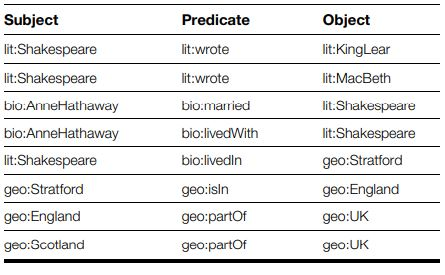
\includegraphics[scale=0.75]{img/RDF escrit R.JPG}
\caption{Tabla de Triples que se refieren a URIs con diversos namespaces. \cite{b1}}
\end{figure}

\subsection{Namespaces Estándar}

El W3C (World Wide Web Consortium) define una serie de namespaces estándar para usarse con tecnologías Web, esto incluye $xsd:$ para la definición de esquemas XML; $xmls:$ para namespaces XML; entre otros.
De manera que usaremos qnames para referirnos a estos términos, utilizando las siguientes definiciones para el estándar de namespaces:

\begin{itemize}
    \item $rdf$: indica identificadores usdos en RDF. El URI global para el namespace $rdf$ es \url{http://www.w3.org/1999/02/22-rdf-syntax-ns\#}\cite{b2}.
    \item $rdfs$: indica identificadores usados para el lenguaje de esquemas RDF, RDFS. El URI global para el namespace $rdfs$ es \url{http://www.w3.org/2000/01/rdf-schema\#}\cite{b3}.
    \item $owl$: indica identificadores usados para el lenguaje de ontología web, OWL. El URI global para el namespace de $owl$ es \url{http://www.w3.org/2002/07/owl\#}\cite{b4}.
\end{itemize}

Estos URI son un buen ejemplo de la interacción entre URI y URL.

\subsection{Identificadores en el namespace de RDF y RDF Schema}

El modelo de datos RDF especifica la noción de triples y la idea de fusionar conjuntos de triples como ya lo hemos apreciado; además RDF usa la infraestructura de la Web para referirse a alguna entidad particular.
El estándar RDF usa la infraestructura del namespace para definir una pequeña cantidad de identificadores estándar en un namespace llamado $rdf$.

\texttt{rdf:type} es una propiedad que proporciona un sistema de escritura elemental en RDF. Por ejemplo se puede expresar relaciones entre varios dramaturgos al usar la información del tipo ($type$) como se muestra en la siguiente tabla:


\begin{figure}[H]
\centering
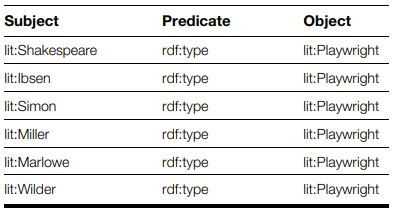
\includegraphics[scale=0.75]{img/RDF tabla type 1-1.JPG}
\caption{Tabla donde se usa $rdf$ para describir dramaturgos. \cite{b1}}
\end{figure}

El sujeto de \texttt{rdf:type} en estas triples puede ser cualquier identificador, y el objeto se puede entender como un tipo ($type$).
Estrictamente no hay límites en el uso de \texttt{rdf:type} pues los tipos pueden tener más tipos.


\texttt{rdf:Property} es un identificador que es usado como un tipo en RDF que indica cuando otro identificador debe usarse como predicado en lugar de usarse como sujeto u objeto.
Como dato curioso podemos declarar todos los identificadores que se han usado hasta ahora como predicados tal como se muestra en la siguiente tabla.

\texttt{rdf:subClassOf} es una instancia de \texttt{rdf:Property} que se utiliza para indicar que todas las instancias de una clase son instancias de otra.

\subsection{RDF y datos tabulares}

Ahora que tenemos los mecanismos sobre RDF el cual es una forma de distribuir datos a través de la Web, podemos retomar los datos tabulares y mostrar cómo representarlos de forma coherente en RDF.

\subsubsection{Desafío}

Se tiene una base de datos relacional que describe los personajes de la serie animada One Punch Man la cual fue tomada de este sitio web: \url{https://onepunchman.fandom.com/es/wiki/Portada}\cite{b5}

 Realizar un grafo que refleje el contenido de la base de datos de tal manera que se conserve el propósito de la información, pero con los datos aptos para realizar operaciones RDF como fusión y consulta RDF.

\textbf{Solución}

Cada personaje en la página web describe una entidad, todas del mismo tipo. Entonces el tipo esta dado por el nombre de los personajes, $Personajes$.

Conocemos información sobre cada elemento según el contenido de la web, como el nombre, alias, asociación, etc. por lo que queremos representar esta información en RDF.

Cada personaje tendrá un URI porque representa una única entidad. Por suerte la necesidad de un identificador único esta presente en la base de datos al igual que en la Web Semántica, por lo que cuenta con  un identificador único válido (el hipervínculo de cada personaje p.e. \url{https://onepunchman.fandom.com/es/wiki/Saitama}\cite{b6}).

La forma más sencilla para formar un identificador de este tipo es tener un solo URI para la base de datos. Como esta es una base de datos de una página web vamos a llamar al namespace $n:$.

Entonces podemos crear un identificador para cada línea concatenando el nombre de los personajes, $Personajes$ con la clave única y expresando este identificador en el namespace $n$, dando como resultado los identificadores \texttt{n:Personaje1, n:Personaje2}
y así sucesivamente. 

Como cada fila contiene diversa información de cada elemento, se usa alguna propiedad que describa al producto. Pero al igual que en el caso de las filas, necesitamos identificadores únicos globales para las propiedades.

Para evitar confusiones se combina el nombre de la tabla y el nombre de la columna, esto da como resultado propiedades como
\texttt{n:Personaje\_Alias, n:Personaje\_Categoría} y así.

Establecido lo anterior, habrá un triple por celda en la tabla; es decir, para $n$ filas y $c$ columnas habrá $n$x$c$ triples.

%En la Figura 15 cada fila corresponde a un producto, esto se puede representar en RDF al agregar un 
%triple por fila que especifique el tipo de individuo descrito por cada fila como se muestra en la Figura 17.

\begin{table}[H]
\begin{center}
\begin{tabular}{|c|c|c|}
\textbf{Subject}& \textbf{Predicate} & \textbf{Object}  \\
     n:saitama & n:Es & Héroe \\
     n:saitama & n:Alias & Pelado con capa\\
     n:saitama & n:Literal & Héroe \\
\end{tabular}
\end{center}
\caption{Tabla de triples que representan algunos de los datos de la base de datos.}
\end{table}


En el caso de la data en RDF que nosotros estamos manejando, haremos uso del servicio que presta la siguiente página web para poder observar el grafo obtenido: \url{https://www.ldf.fi/service/rdf-grapher}\cite{b7}


\subsubsection{Relaciones de orden superior}

Para anexar más información a un \texttt{Triple} de un RDF se usa la cosificación, la cual permite matizar la data; en otras palabras, realizar una declaración sobre otra declaración y así sucesivamente.

\subsection{Alternativas de serialización}

Existen formas de expresar RDF en forma textual, sin embargo, usaremos la forma RDF / XML.

\subsubsection{RDF / XML}

Esta manera de expresar el RDF es para facilitar la representación de información en HTML, de manera general, XML.

Podemos encontrar más información en \url{http://www.w3.org/TR/rdf-syntax-grammar/} \cite{b8}


\section{Descripción de recursos usando RDF}

Para este trabajo se han añadido características de cada personaje; es decir, una concatenación de predicados para formar triples de grado superior.

\begin{itemize}
    \item Ocupación: define si el personaje es un héroe, villano u otro.
    \item Clases"X": son las clases a las que pertenecen los personajes Héroes, presentan las categorías: S, A, B, C; así como la de los monstruos como Dragón, Tigre, etc.
    \item Organizaciones: son los "grupos principales" a los que pertenece un personaje.
    \item Técnicas: hace referencia a las técnicas que puede tener o no un personaje.
    \item Nombre litera: son los nombres literales de los personajes, técnicas, etc. que tenga un nombre propio.
    \item Características generales: son especificaciones de los personajes como Alias, rango, entre otros.
\end{itemize}

Además, para este trabajo de investigación se hizo uso de las siguientes tecnologías:

\begin{itemize}
    \item ipython notebooks: son documentos de cuaderno en el que se permite ejecutar segmentos de código de manera separada.
    \item rdflib: es una librería o módulo que usa python para trabajar con RDF.
    \item git: es un sistema de control de versiones.
    \item github: es un servicio de hosting para almacenar repositorios en internet.
    \item RDF Grapher: es un servicio web para analizar datos RDF y visualizarlo como un gráfico.
\end{itemize}

\section{Manipulación de RDF}

Primero se realizó la configuración del entorno de trabajo, importando las librerías y elementos de la librería que sean necesario.

Se crea el namespace principal, en este caso lo llamamos $n$ el cual es la URL de la página de donde se obtiene la información.

Posterior a ello se realizó la creación de \texttt{qnames} para los personajes, localizaciones, asociaciones, técnicas, etc. con sus respectivos URI referenciados en la web.

Se crean \texttt{qnames} de algunas características propias con una URI local.

Se crea el grafo, el cual es un elemento de la librería $rdflib$, al cual llamaremos grafo $g$.

Al tener todos los datos referenciados, se procede a realizar la agregación de información al grafo $g$, se hace uso de los identificadores rdf:type, rdfs:subClassOf, entre otros; construyendo así las relaciones entre las entidades que contendrá el grafo. 

A medida que se van añadiendo personajes (sujeto) al grafo, se les agrega sus características (predicado y objeto). De esta manera se van organizando uno por uno.

Finalmente podemos comprobar la integridad de nuestro grafo al serializarlo en el formato $XML$.
Como resultado obtendremos un código en XML el cuál llevaremos al servicio de la página RDF Grapher para poder visualizar el grafo generado.

\subsection{Inferencias}

Las inferencias son una forma de navegación en el RDF. Para realizar una usaremos una función que reciba una subclase, una superclase y el grafo al que pertenecen.
En ellas se comprobará si la subclase es igual a la superclase, en dicho caso, se devolverá \texttt{TRUE} pues esta subclase está incluida en sí misma. Caso contrario se buscará en cada parentezco que tenga la subclase hasta encontrar la coincidencia para devolver \texttt{TRUE}.
De no tener coincidencias se devolverá \texttt{FALSE} pues se infiere que no hay parentezco entre ambas clases; es decir, no es subclase de nuestra superclase en dicho grafo.

% describe las clases (p.e. ClaseB representa a un personaje que pertenece a la asociación de héroes)
%insertar personajes y uri
% creación de estructura base del grafo
% clases personajes -> subclases (heroes villanos aliens) -> subclases sucesivas
% se agrega el personaje al  grafo y se usa rdf:type para relacionar a la subclase a la que pertenece

\section{Conclusiones}
    
    \begin{itemize}
        \item Se ha logrado comprender el funcionamiento y utilidad del uso de RDF.
        \item Se ha podido realizar una inferencia y se ha respondido correctamente.
    \end{itemize}




\begin{thebibliography}{00}
\bibitem{b1}ALLEMANG, D., HENDLER, J. (2011). Semantic web for the working ontologist: effective modeling
in RDFS and OWL (2 nd edition). \href{https://doi.org/10.1016/C2010-0-68657-3}{Enlace}.
\bibitem{b2}W3 organization \url{https://www.w3.org/1999/02/22-rdf-syntax-ns#}
\bibitem{b3}W3 organization \url{http://www.w3.org/2000/01/rdf-schema#}
\bibitem{b4}W3 organization \url{http://www.w3.org/2002/07/owl#}
\bibitem{b5}One Punch Man fandom \url{https://onepunchman.fandom.com/es/wiki/Portada}
\bibitem{b6}One Punch Man fandom - Personaje: Saitama \url{https://onepunchman.fandom.com/es/wiki/Saitama}
\bibitem{b7}ldf: visualizador de grafos \url{https://www.ldf.fi/service/rdf-grapher}
\bibitem{b8}W3 organization - syntaxis de rdf \url{http://www.w3.org/TR/rdf-syntax-grammar/}
\end{thebibliography}

\end{document}